
\chapter{QUADRO METODOLÓGICO}
\label{cap:quadroMetodologico}


\par Neste quadro metodológico serão apresentados os passos que se fizeram necessários para a realização desta pesquisa. Nele estão descritos desde a escolha do perfil da pesquisa até os procedimentos utilizados para o seu desenvolvimento. \citeonline{gil_metodos_e_tecnicas_de_pesquisa}, cita que a metodologia é um conjunto de procedimentos intelectuais e técnicos que trabalham para a realização do objetivo proposto.
\par Posterior ao estudo do levantamento teórico e técnico, foram definidos os procedimentos para a construção deste trabalho, iniciando pela escolha do tipo de pesquisa, demonstrada na seção a seguir.


%Será apresentado neste capítulo a metodologia de pesquisa a ser utilizada para a realização deste projeto e os passos necessários até a sua conclusão.

\section{Tipo de pesquisa}

\par Para \citeonline[p. 31]{padua_metodologia_pesquisa}, pesquisa é:

\begin{citacao}
	Toda atividade voltada para a solução de problemas; como atividade de busca, indagação, investigação, inquirição da realidade, e a atividade que visa nos permitir, no âmbito da ciência, elaborar um  conhecimento, ou um conjunto de conhecimentos, que nos auxilie na compreensão desta realidade e nos oriente em nossas ações.
\end{citacao}

% Comentário, pois estava repetindo demais o fato de utilizar  apesquisa aplicada no desenvolvimento do trabalho. 
%\par O tipo de pesquisa aplicada foi escolhido para o desenvolvimento da pesquisa, pois conforme \citeonline[p. 32]{cooper_schindler_metodos_pesquisa_administracao}, ela ``tem uma ênfase prática na solução de problemas, embora a solução de problemas nem sempre seja gerada por uma circunstância negativa.''

\par De forma objetiva, a pesquisa é o meio utilizado para buscar respostas aos mais diversos tipos de indagações, tendo por base procedimentos racionais e sistemáticos. A pesquisa é realizada quando se tem um problema e não se têm informações suficientes para solucioná-lo. Por meio desta sessão, tem-se como objetivo explicar o tipo de pesquisa que norteou o desenvolvimento deste trabalho, justificando também como ele se enquadra no tipo escolhido.

\par Pesquisar é um trabalho que envolve planejamento, para que ela seja satisfatória, o pesquisador precisa estar envolvido e  desenvolver habilidades técnicas que o levem a escolher o melhor caminho em busca da obtenção dos resultados.

\par Segundo \citeonline{fonseca_metodologia_da_pesquisa}, ter um método de pesquisa envolve o estudo dos fatores que compõem o contexto da pesquisa, tais como, a escolha do caminho e o planejamento do percurso. Essa escolha inicia-se com a definição do tipo de pesquisa utilizada. Para este trabalho, é utilizada a pesquisa aplicada, que é aquela cujo o pesquisador tem como objetivo aplicar os conhecimentos obtidos durante o período da pesquisa, em um projeto real, a fim de conhecer os seus resultados. \citeonline{gil_como_elaborar_projeto_de_pesquisa} afirma que este tipo de pesquisa dirige-se à solução de problemas específicos, de interesses locais.

%\par Conforme \citeonline[p. 32]{cooper_schindler_metodos_pesquisa_administracao}, a pesquisa aplicada tem uma ênfase prática na solução de problemas. 
\par Nesta pesquisa foram estudados os conceitos de banco de dados orientado à grafos e a sua aplicabilidade, desenvolvendo, por meio dos conhecimentos obtidos pela pesquisa, uma solução prática, disponibilizada por meio de um sistema \textit{web}, que auxilia na busca por mão de obra temporária, que não caracterize vínculo empregatício.

\par Seguindo o enquadramento desta pesquisa, ela deve ser aplicada a um contexto específico, conforme será abordado a seguir. 



%\par Seguindo esta ideia, este tipo de pesquisa será utilizado no desenvolvimento deste projeto, pois, o objetivo é gerar uma solução para o problema de localização de mão de obra, por meio de um sistema \textit{web}. Este projeto adequa-se perfeitamente ao tipo de pesquisa aplicada, uma vez que o mesmo busca analisar e gerar uma possível solução para o problema em destaque.

%Parágrafo utilizado no pré-projeto. Foi corrigido por Edilson no dia 02/04/15 e criado o parágrafo acima
%\par Este tipo de pesquisa será utilizada no desenvolvimento deste projeto, pois a mesma busca analisar o problema e gerar uma solução para o mesmo através de um aplicativo ou serviço.  Neste caso, será o desenvolvimento de um sistema \textit{web} que auxilia na busca por profissionais temporários.


\section{Contexto de pesquisa}
\par O trabalho informal é um elemento estrutural da economia no Brasil e nos países em desenvolvimento. Ele faz parte do cenário atual, crescente a cada dia, e contribui ativamente com a geração de renda. É considerado como um desdobramento do excesso de mão de obra, definido a partir de pessoas que criam sua própria forma de trabalho como estratégia de sobrevivência ou como forma alternativa de recolocação no mercado de trabalho. O fortalecimento deste tipo de trabalho ocorre a partir da construção de redes, formadas por parentes e amigos, criando laços de confiança que são fundamentais para o desempenho da atividade. No entanto, há uma grande dificuldade em se encontrar estes profissionais, uma vez que não há um lugar centralizado para divulgar o seu perfil profissional.

\par O desenvolvimento deste trabalhos se propôs atuar sob essa limitação. Uma pesquisa informal, realizada no sul de Minas Gerais, com pessoas de diferentes perfis sociais, constatou que uma aplicação, capaz de centralizar a busca por estes profissionais, seria muito bem aceita. A partir deste resultado, validou-se a ideia de construir um ambiente \textit{web} onde o trabalhador informal tem o espaço para centralizar suas habilidades e manter um perfil visível aos possíveis contratantes. Qualquer prestador de serviço informal pode ter acesso a este ambiente, desde que possua um dispositivo eletrônico capaz de se conectar a internet. 

\par O ambiente desenvolvido também visa facilitar ao contratante, a busca por estes profissionais, uma vez que não é fácil localizá-los por meio dos mecanismos de busca tradicionais. Desta forma existe um benefício mutuo, onde contratados e contratantes se despõem da praticidade.

\par Enfim, o contexto ao qual esta pesquisa se destina busca ser bem abrangente, com o intuito de contribuir de forma relevante, proporcionando uma boa experiência aos envolvidos.
 
%Exemplo de contexto que a Joelma deu na sala de aula. Usar como exemplo
%\par Este sistema volta-se para implantação e execução em todas as empresas de pequeno porte do ramo varejista no sul de minas gerais que tenha apresentado a necessidade de um controle mais rigoroso da sua entrada e saída de mercadorias

%Segundo a Joelma e o Márcio este seria o contexto da pesquisa: As pessoas que buscam mão de obra para determinados tipos de trabalho (contratantes) e as pessoas que disponibilizam tais mãos de obra (contratados ou prestadores de serviços).

%Antigo Contexto que a Joelma disse que estava muito geral na correção do pré-projeto
%\par Esta pesquisa terá como foco todas as pessoas que necessitam de mão de obra temporária para realizar tarefas domésticas e rotineiras, além daquelas que não ocorrem com tanta intensidade. Uma vez que o sistema será desenvolvido em uma plataforma \textit{web}, todas as pessoas terão fácil acesso ao serviço, sendo necessário apenas possuir uma comunicação com a internet.

%\par Esta pesquisa terá como foco todas as pessoas da região do sul de Minas Gerais, que necessitam de determinados tipos de mão de obra (contratantes), bem como para aqueles que necessitam de um espaço para divulgar esta oferta (contratados ou prestadores de serviços). Tomando por base que encontrar este tipo de profissional tem se tornado uma tarefa cada vez mais complicada, que acaba gerando transtornos na vida da população, pois, em muitos casos, a falta de opções leva a contratações equivocadas e infelizes.

%\par Como o sistema será desenvolvido em uma plataforma \textit{web}, todas as pessoas neste contexto terão fácil acesso ao serviço, permitindo a disseminação desta ferramenta, sendo necessário apenas possuir uma comunicação com a internet.


%\section{Participantes}

\par Participaram desta pesquisa dois acadêmicos e um professor orientador, sendo eles Andressa Faria, Edilson Justiniano e Márcio Emílio.
\par Andressa de Faria Giordano, acadêmica do 7º período do curso de bacharelado em Sistemas de Informação pela Universidade do Vale do Sapucaí - UNIVAS - com formação técnica e profissionalizante pelo Instituto Nacional de Pesquisa Tecnologica e Computacional - INPETTECC. Sua participação, neste projeto, será o levantamento dos requisitos e a elaboração de todos os diagramas descritos nas fases do ICONIX, a modelagem do banco de dados, a implantação da lógica de negócios, comunicação entre os módulos, acesso aos dados pelo sistema e a documentação do trabalho.

\par  Edilson Justiniano, acadêmico do 7º período do curso de bacharelado em Sistemas de Informação pela Universidade do Vale do Sapucaí - UNIVAS - com formação técnica e profissionalizante pelo Instituto Nacional de Pesquisa Tecnologica e Computacional - INPETTECC. Sua participação, neste projeto, será o levantamento dos requisitos e a elaboração de todos os diagramas descritos nas fases do ICONIX, a modelagem do banco de dados, a implantação da lógica de negócios, comunicação entre os módulos, acesso aos dados pelo sistema e a documentação do trabalho.

\par Márcio Emílio Cruz Vono de Azevedo,professor orientador, engenheiro elétrico em modalidade eletrônica pelo Instituto Nacional de Telecomunicações - INATEL - e mestre em Ciência da Computação pela Universidade Federal de Itajubá - UNIFEI. Professor do INATEL e da Universidade do Vale do Sapucaí - UNIVAS - na área de engenharia de \textit{software} e especialista em sistemas do Inatel.


\par A elaboração do texto escrito será realizado com base nas ações que serão desenvolvidas pelos participantes e serão feitas em conjunto.


\section{Instrumentos}

\par Os instrumentos de pesquisa são as ferramentas usadas para a coleta de dados. Como afirma \citeonline[p. 117]{marconi_lakatos_metodologia_trabalho_cientifico}, eles abrangem “desde os tópicos de entrevista, passando pelo questionamento e formulário, até os testes ou escala de medida de opiniões e atitudes”. Eles são de suma importância para o desenvolvimento de um projeto, pois visam a levantar o máximo de informações possíveis para nortear as tomadas de decisões. Para a realização desta pesquisa foram utilizados questionários e análise documental.

\par Segundo \citeonline{gil_como_elaborar_projeto_de_pesquisa}, o questionário é um dos procedimentos mais utilizados para obter informações, pois é uma técnica de custo razoável, apresenta as mesmas questões para todas as pessoas, garante o anonimato e pode conter as questões para atender a finalidades específicas de uma pesquisa. Se aplicada criteriosamente, essa técnica apresenta elevada confiabilidade. Os questionários podem ser desenvolvidos para medir opiniões, comportamento, entre outras questões, também pode ser aplicada individualmente ou em grupos.

\par Para este trabalho, foi desenvolvido um questionário informal, aplicado de forma individual, disponibilizado no ambiente virtual, o qual foi respondido com o intuito de analisar se a pesquisa aqui pretendida seria bem aceita por pessoas de diferentes perfis sociais. %A seguir são discriminados os resultados obtidos.

%Aqui colocar o resultado da análise do questionário

\par A análise documental consiste em identificar, verificar e apreciar os documentos, atendendo a uma finalidade específica, que visa extrair uma informação objetiva da fonte. Para este trabalho foi utilizada a análise documental como material de apoio, que norteou tanto o desenvolvimento teórico quanto o prático.

\par Feita a escolha dos instrumentos, foram definidos os procedimentos necessários para que a pesquisa fosse realizada. Estes procedimentos serão descritos na próxima seção.




%\subsection{Questionários}

\par Para \citeonline{silva_menezes_metodologia_pesquisa_elaboracao_dissertacao}, questionário é:

\begin{citacao}
	Uma série ordenada de perguntas que devem ser respondidas por escrito pelo informante. O questionário deve ser objetivo, limitado em extensão e estar acompanhado de instruções As instruções devem esclarecer o propósito de sua aplicação, ressaltar a importância da colaboração do informante e facilitar o preenchimento.
\end{citacao}

%\par Qual o objetivo de aplicar o questionário? Serão aplicados os questionários para a empresa tal, a fim de levantar o grau de satisfação dos funcionários com o sistema.

%\par Quantos ou quantas e para quem?

\par Serão disponibilizados questionários \textit{on-line} a fim de avaliar o interesse da população por um sistema que ofereça o serviço de localização de mão de obra temporária. Para desenvolver tal \textit{software}, uma bateria de testes será feita visando oferecer a melhor interação entre o usuário e o software, levando em conta sua aplicabilidade, desempenho e facilidade de utilização.

%\par A observação será feita através de formulários de pesquisa que avaliarão o interesse dos usuários pelo sistema que ofereça o serviço de localização de mão de obra temporária. Os testes serão feitos visando oferecer a melhor interação entre o usuário e o software, levando em conta sua aplicabilidade, desempenho e facilidade de utilização.


%Reunião não é aplicado ao nosso trabalho pq reunião não é um instrumento de pesquisa
%\section{Reuniões}

%\par Serão realizados encontros presenciais e também virtuais com os acadêmicos e com o professor orientador, para o levantamento dos requisitos, da aplicabilidade do software, dos modelos de engenharia de software e codificação do sistema, como também questões teóricas que estejam relacionadas com as melhores práticas para se obter um software aplicável e ágil.


%\subsection{Análise documental}

\par Para auxiliar no desenvolvimento deste projeto serão utilizados documentos como: manuais, tutoriais, livros, trabalhos e artigos acadêmicos, além de pesquisa web. Estes serão utilizados para o embasamento teórico que consiste no levantamento de requisitos e tecnologias a serem abordadas, e também para o desenvolvimento prático servindo como apoio e referencial para futuras consultas.


\section{Procedimentos}

\par Para que esta pesquisa fosse levada a cabo, tornou-se necessário a implementação de algumas ações, as quais serão detalhadas.

\par O início da pesquisa deu-se através da escolha do tema, seguido pelo levantamento das tecnologias que seriam utilizadas. A princípio, foi definido um escopo contendo algumas tecnologias que foram ministradas no ambiente acadêmico, o que diminui a curva de aprendizado, no entanto, foi preciso agregar alguns conhecimentos novos, onde foi desprendido um tempo a mais para estudo e realização de pequenos testes. As tecnologias que foram empregadas no desenvolvimento deste trabalho são as seguintes: a linguagem de programação JAVA, o banco de dados orientado a grafos Neo4j, juntamente com a API Cypher, Tomcat, Primefaces e JSF, sendo que no decorrer do desenvolvimento prático, viu-se a necessidade de substituir as duas ultimas tecnologias citadas pelas linguagens HTML, CSS, Javascript e Angular JS. As tecnologias que acompanharam o desenvolvimento deste trabalho até a sua conclusão estão descritas no quadro teórico desta pesquisa.

\par Para garantir que as tecnologias selecionadas seriam a melhor escolha no desenvolvimento deste trabalho, foram realizados alguns testes por meio de aplicações simples. Os testes foram focados na avaliação do comportamento do banco de dados orientado a grafos aplicado ao contexto desta pesquisa, cujo objetivo foi desenvolver uma aplicação de busca de mão de obra baseada em uma rede de relacionamentos. Estes testes também foram realizados como fins didáticos, a fim de se familiarizar com as tecnologias utilizadas.

\par Para garantir a qualidade desta pesquisa, o ICONIX foi escolhido como a metodologia de desenvolvimento de \textit{software}, desempenhando um papel fundamental na organização do trabalho. Sua abordagem proveu uma sequencia de procedimentos, que foram seguidos conforme o necessário, levando a construção de uma aplicação estável. Como relatado no quadro teórico, foram seguidas as quatro fases definidas pelo ICONIX.

\par Na primeira fase, definida como análise de requisitos, foi realizado o levantamento das informações pertinentes ao desenvolvimento da aplicação. Este levantamento foi realizado por meio da observação do comportamento das pessoas ao realizar essa busca por mão de obra temporária. A partir dai, foram levantadas as principais características, que seriam indispensáveis para o desenvolvimento deste trabalho e criado o modelo de domínio inicial do projeto como demonstra a Figura 15, com base nas informações levantadas. Nesta fase também foram definidas todas as ações que o usuário poderia realizar no sistema, por meio dos casos de uso, conforme a Figura 16.

\newpage
\begin{figure}[h!]
	\centerline{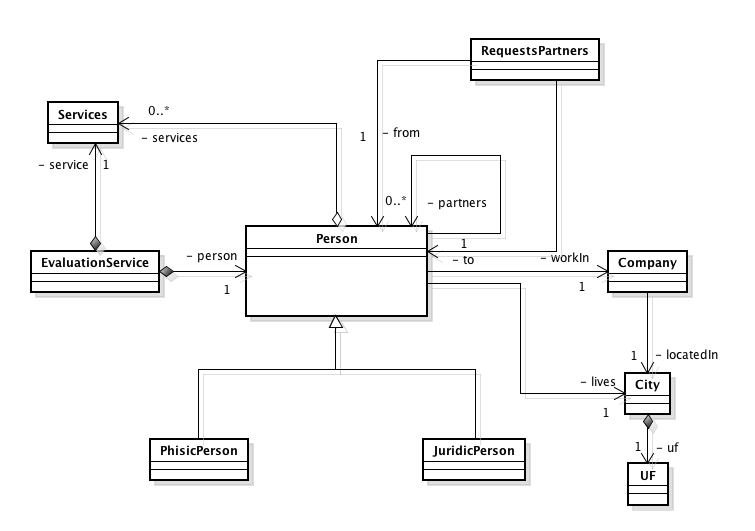
\includegraphics[scale=0.45]{./imagens/modelo-dominio-inicial.png}}
	\caption[Modelo de domínio inicial]
	{Modelo de domínio inicial. \textbf{Fonte:} Elaborado pelos autores.}
	\label{fig:exemplo1}
\end{figure}

\begin{figure}[h!]
	\centerline{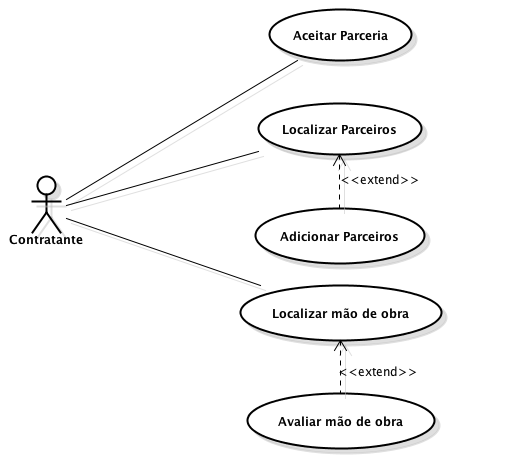
\includegraphics[scale=0.6]{./imagens/caso-de-uso.png}}
	\caption[Diagrama de caso de uso]
	{Diagrama de caso de uso. \textbf{Fonte:} Elaborado pelos autores.}
	\label{fig:exemplo1}
\end{figure}

\par Na segunda fase, análise e projeto preliminar, houve um refinamento dos requisitos levantados na fase anterior, definindo melhor as ações do usuário, por meio dos diagramas de casos de uso. Posterior a esta definição foram gerados os diagramas de robustez, de acordo com os casos de uso definidos, como demonstra a Figura 17. Paralelamente a modelagem desses diagramas, foi atualizado o modelo de domínio, acrescentando os atributos identificados, conforme a Figura 18. Com o modelo de domínio atualizado, foi feita a modelagem do banco de dados da aplicação como apresenta a Figura 19.

\begin{figure}[h!]
	\centerline{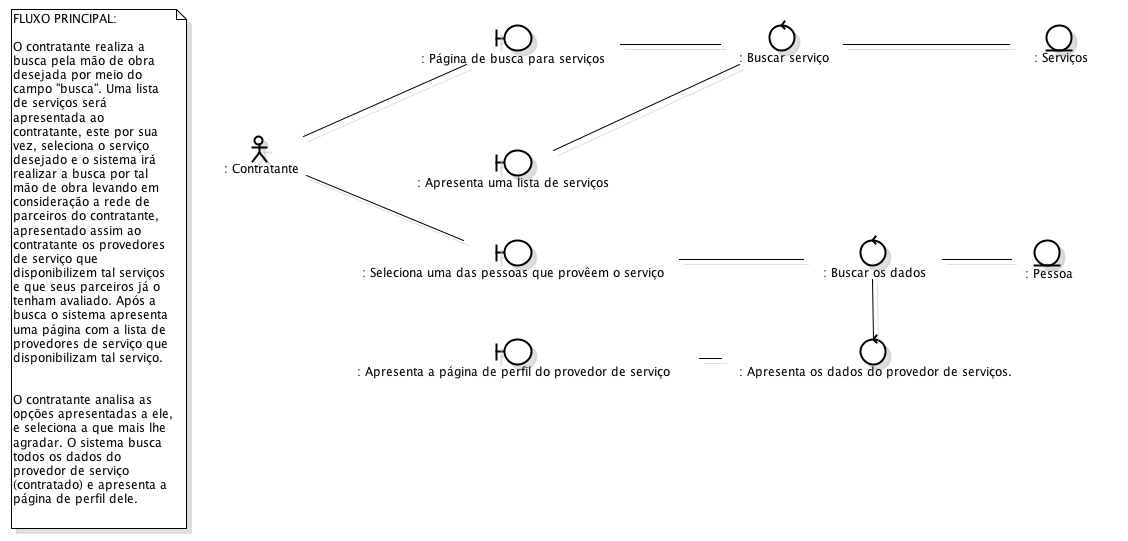
\includegraphics[scale=0.35]{./imagens/robustez.png}}
	\caption[Diagrama de robustez do caso de uso Localizar mão de obra]
	{Diagrama de robustez do caso de uso Localizar mão de obra. \textbf{Fonte:} Elaborado pelos autores.}
	\label{fig:exemplo1}
\end{figure}

\begin{figure}[h!]
	\centerline{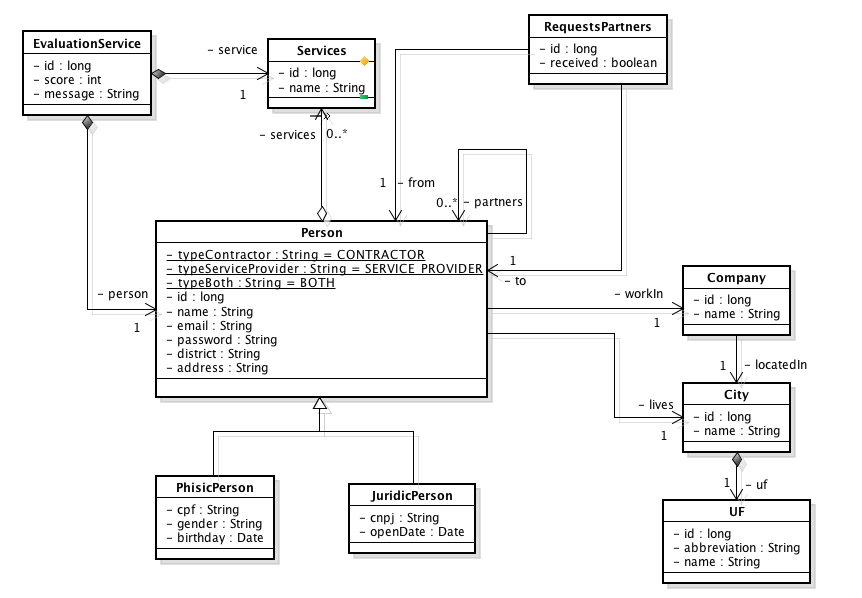
\includegraphics[scale=0.6]{./imagens/modelo-dominio-com-atributos.png}}
	\caption[Modelo de domínio atualizado]
	{Modelo de domínio atualizado. \textbf{Fonte:} Elaborado pelos autores.}
	\label{fig:exemplo1}
\end{figure} 

\begin{figure}[h!]
	\centerline{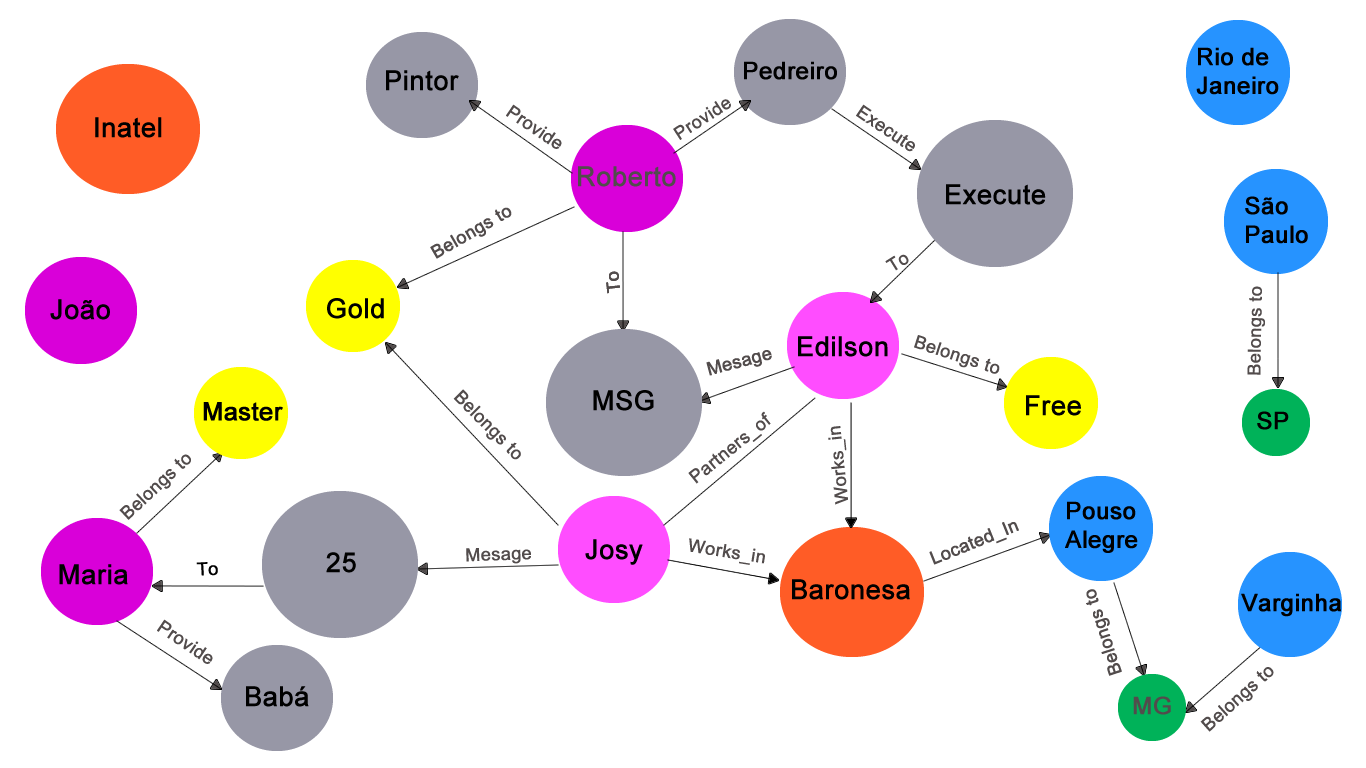
\includegraphics[scale=0.5]{./imagens/structure-all-nodes.png}}
	\caption[Modelo de dados da aplicação]
	{Modelo de dados da aplicação. \textbf{Fonte:} Elaborado pelos autores.}
	\label{fig:exemplo1}
\end{figure} 


\par Na terceira fase, definida como projeto detalhado, foram criados os diagramas de sequencia, tendo como base os casos de uso modelados na fase anterior. Esta fase tem como objetivo detalhar todo o funcionamento do \textit{software}, visando definir a melhor maneira de realizar sua implementação. A Figura 20 apresenta o diagrama de sequência do caso de uso localizar mão de obra.

\newpage
\begin{figure}[h!]
	\centerline{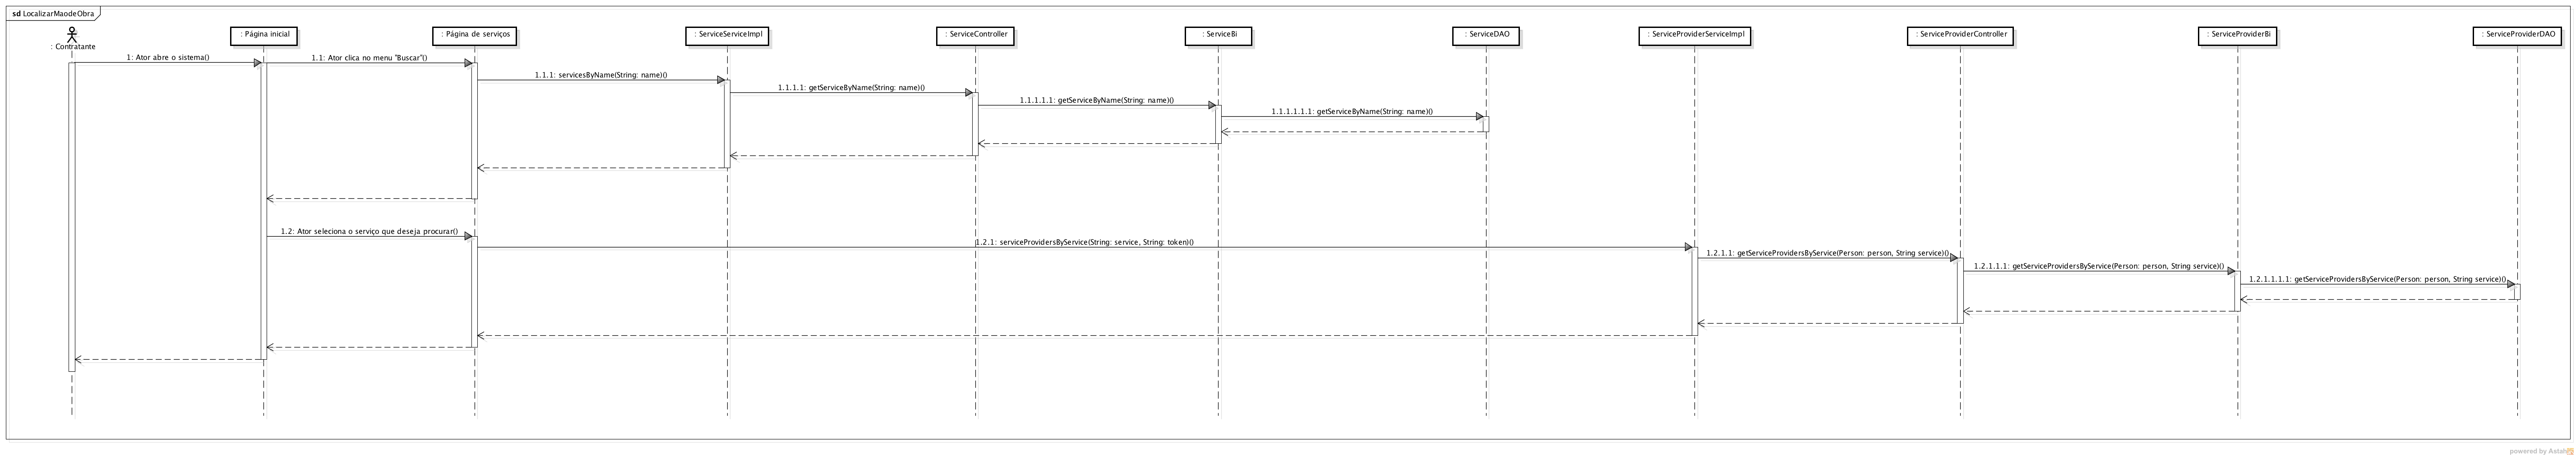
\includegraphics[angle=90,height=0.7\textheight,width=0.7\textwidth]{./imagens/sequence-localizar-mao-de-obra.png}}
	\caption[Diagrama de caso de uso]
	{Diagrama de caso de uso \textbf{Fonte:} Elaborado pelos autores.}
	\label{fig:exemplo1}
\end{figure}

\par Ainda na fase de projeto detalhado, após a modelagem dos diagramas de sequencia, as operações encontradas nestes diagramas foram adicionadas ao modelo de domínio, em conjunto com as novas classes identificadas, gerando assim, o digrama de classes.

imagem do diagrama de classes


\par Na quarta e última fase do ICONIX, denominada implementação, iniciou-se a preparação do ambiente de desenvolvimento, incluindo a instalação de \textit{softwares} adicionais, necessários para o desenvolvimento prático da aplicação.

\par Visto que o trabalho seria desenvolvido em equipe, foi necessário estabelecer uma ferramenta de controle de versão. Esta ferramente permitiu o gerenciamento de diferentes versões de arquivos, gerando um histórico contendo as modificações que foram realizadas no decorrer do processo de desenvolvimento. Este histórico permite o retorno de alguma revisão, caso haja necessidade. A ferramenta escolhida para realizar esse controle foi o GitHub, que já havia sido utilizado em alguns trabalhos do contexto acadêmico, evitando o desprendimento de tempo para estudo de uma nova ferramenta de apoio. O GitHub é uma ferramenta bem difundida e permite que os seus usuários colaborem com os projetos que estão armazenados em seus repositórios\footnotemark[31]. A Figura 21 demonstra a tela de serviços provida pelo GitHub.

\footnotetext[31]{Repositório: local cujo desenvolvedor utiliza para armazenar os documentos relacionados ao \textit{software}.}

\begin{figure}[h!]
	\centerline{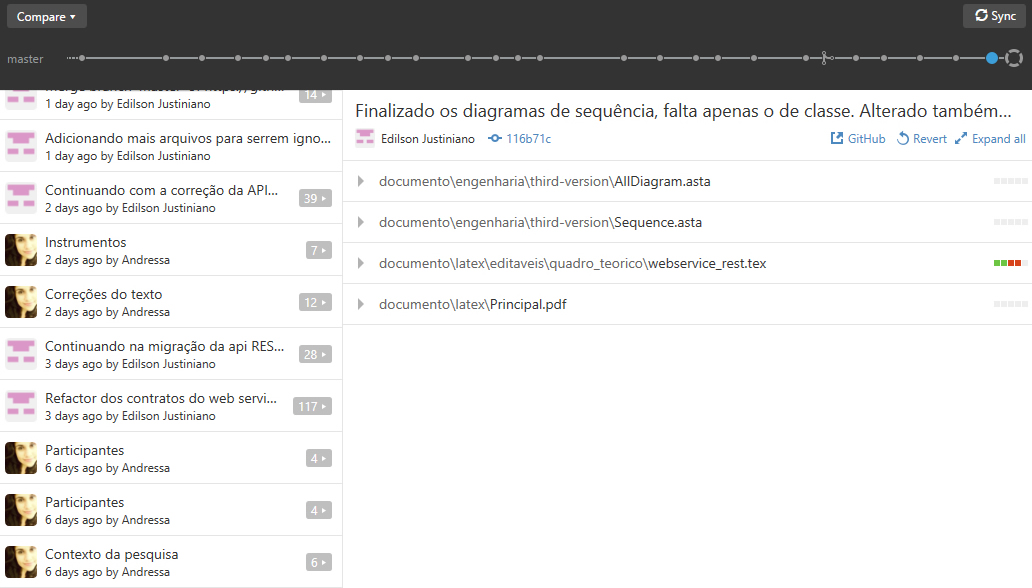
\includegraphics[scale=0.35]{./imagens/github.jpg}}
	\caption[Tela de serviços do GitHub ]
	{Tela de serviços do GitHub \textbf{Fonte:} Elaborado pelos autores.}
	\label{fig:exemplo1}
\end{figure}

\par Os passos de instalação detalhados do GitHub são descritos na sessão apêndices deste trabalho.

\par Como mencionado no quadro teórico, neste trabalho foi utilizada a linguagem Java, sendo assim necessário a utilização de uma IDE de apoio. A IDE escolhida foi o Eclipse, pois se trata de uma ferramenta \textit{open source}, bem difundida no mercado e que permite a escrita de um código mais legível, facilitando tarefas como \textit{debug} e configurações do projeto.

\par O Eclipse possui várias ferramentas, dentre elas, pode-se citar o editor de texto, utilizado não somente para a escrita de códigos em Java, e também a perspectiva de configuração para servidores \textit{web}, utilizada neste trabalho, conforme apresenta a Figura 22. Por meio desta perspectiva, foi configurada a aplicação \textit{container} Tomcat na versão 7.

\newpage
\begin{figure}[h!]
	\centerline{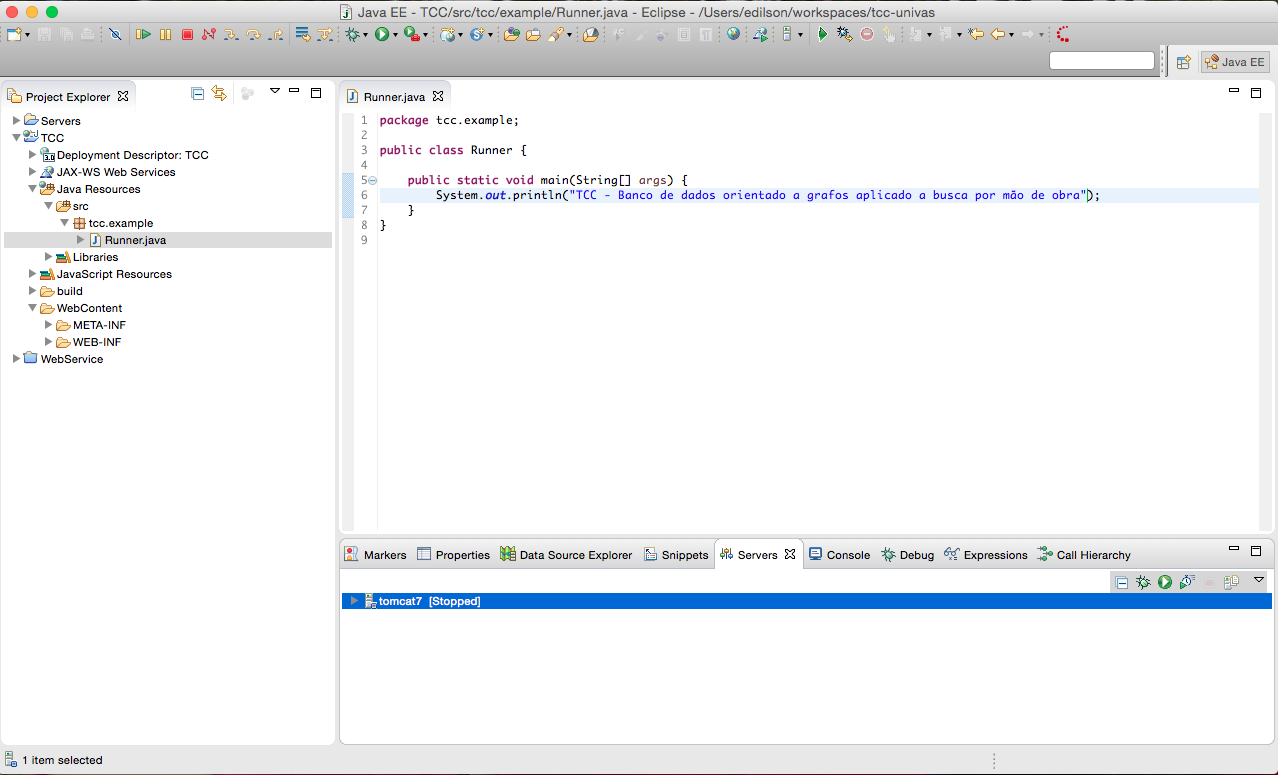
\includegraphics[scale=0.35]{./imagens/eclipse-editor-texto.png}}
	\caption[Ferramentas da IDE Eclipse]
	{Ferramentas da IDE Eclipse \textbf{Fonte:} Elaborado pelos autores.}
	\label{fig:exemplo1}
\end{figure}

\par O Tomcat desempenhou um papel fundamental na execução desta aplicação, pois serviu como hospedeiro para a aplicação Java desenvolvida neste trabalho. 

\par Os passos de instalação e configuração do Eclipse e do Tomcat são descritos na sessão apêndices deste trabalho.

\par Para a escrita do código relacionado ao HTML, CSS e Javascript, foi utilizado o mesmo editor de texto citado anteriormente.

\par O trabalho fez uso de um banco de dados orientado a grafos, o Neo4j. A escolha desse banco se deu pela sua simplicidade de instalação, configuração, facilidade de integração com a API \textit{Cypher} e por disponibilizar uma API REST para acesso aos seus dados, conforme descrito no quadro teórico deste trabalho. O Neo4j faz parte do enquadramento de softwares livres, seguindo o conceito \textit{open source}, o que permite ao desenvolvedor utilizá-lo da forma que melhor lhe convém. 


\par A seguir serão detalhados os passos para a instalação do banco de dados Neo4j.

\par Para realizar o \textit{download} do instalador do banco de dados Neo4j, deve-se acessar a seguinte url, por meio de um  navegador de internet: http://neo4j.com/download e selecionar a opção desejada. Neste trabalho como já descrito foi utilizada a versão \textit{Community}. A Figura 23 apresenta a página de download do Neo4j.

\newpage
\begin{figure}[h!]
	\centerline{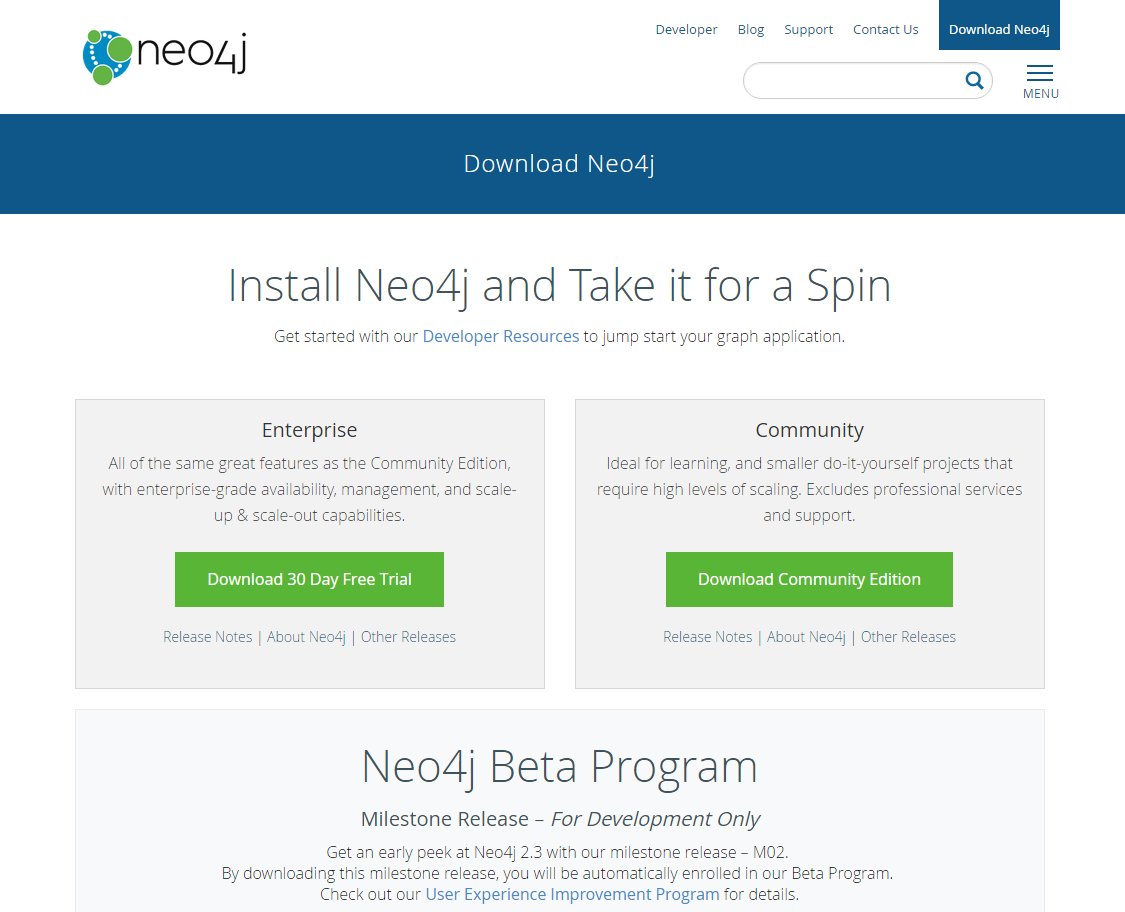
\includegraphics[scale=0.4]{./imagens/download-neo4j.png}}
	\caption[Página de download do Neo4j]
	{Página de download do Neo4j. \textbf{Fonte:} http://neo4j.com/download}
	\label{fig:exemplo1}
\end{figure}

\par Após concluído o \textit{download}, deve-se executar o arquivo. O processo de instalação se inicia e, a primeira tela apresentada ao usuário é a tela contendo uma mensagem de boas vindas, conforme demonstra a Figura 24. Nesta tela, deve-se clicar no botão \textit{Next} para prosseguir com o processo de instalação.

\begin{figure}[h!]
	\centerline{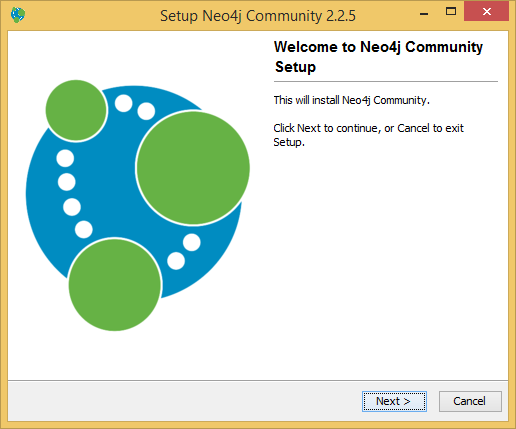
\includegraphics[scale=0.4]{./imagens/neo4j-install-step1.png}}
	\caption[Tela de boas vindas da instalação do Neo4j]
	{Tela de boas vindas da instalação do Neo4j. \textbf{Fonte:} Elaborado pelos autores.}
	\label{fig:exemplo1}
\end{figure}

\par A próxima tela apresentada ao usuário diz respeito ao contrato de uso do \textit{software}, como mostra a Figura 25. Após lê-lo, deve-se aceitar os termos do contrato e clicar no \textit{Next}.

\newpage
\begin{figure}[h!]
	\centerline{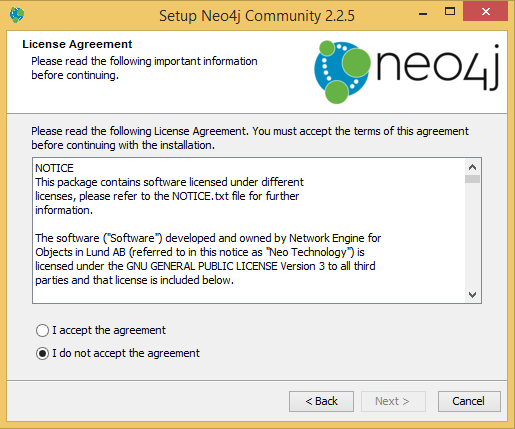
\includegraphics[scale=0.4]{./imagens/neo4j-install-step2.png}}
	\caption[Tela do contrato de uso do Neo4j]
	{Tela do contrato de uso do Neo4j. \textbf{Fonte:} Elaborado pelos autores.}
	\label{fig:exemplo1}
\end{figure}

\par Na próxima tela, conforme a Figura 26 demonstra, é definido o diretório de instalação do Neo4j. Por padrão este diretório é o mesmo das demais aplicações no Windows, podendo ser alterado conforme a necessidade. Após definir o diretório de instalação deve-se clicar no botão \textit{Next}.

\begin{figure}[h!]
	\centerline{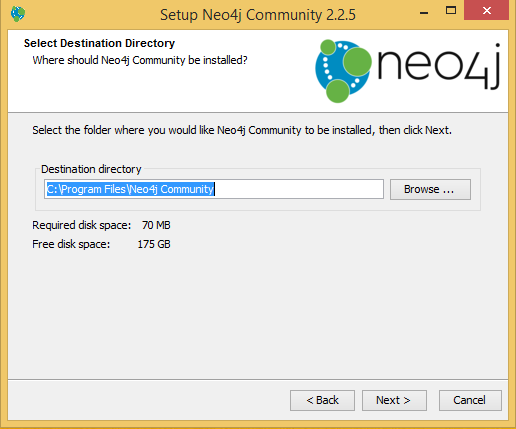
\includegraphics[scale=0.4]{./imagens/neo4j-install-step3.png}}
	\caption[Tela para definição do diretório de instalaão do Neo4j]
	{Tela para definição do diretório de instalaão do Neo4j. \textbf{Fonte:} Elaborado pelos autores.}
	\label{fig:exemplo1}
\end{figure}

\par Após as definições anteriores, uma tela é apresentada questionando ao usuário a respeito da criação de atalhos na área de trabalho, como é demonstrado na Figura 27. Após definir os atalhos do Neo4j, deve-se clicar no botão \textit{Next}.

\begin{figure}[h!]
	\centerline{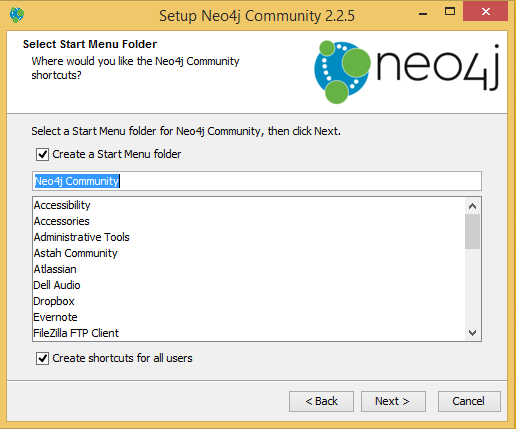
\includegraphics[scale=0.4]{./imagens/neo4j-install-step4.png}}
	\caption[Tela para criação de atalhos do Neo4j]
	{Tela para criação de atalhos do Neo4j. \textbf{Fonte:} Elaborado pelos autores.}
	\label{fig:exemplo1}
\end{figure}

\par Após realizar os procedimentos descritos para a instalação do Neo4j a tela final de instalação será apresentada, informando-o a respeito do resultado da instalação conforme demonstra a Figura 28. Clique no botão \textit{Finish} para finalizar o processo de instalação.
Após todos os passos realizados com sucesso, o Neo4j estará disponível.

\begin{figure}[h!]
	\centerline{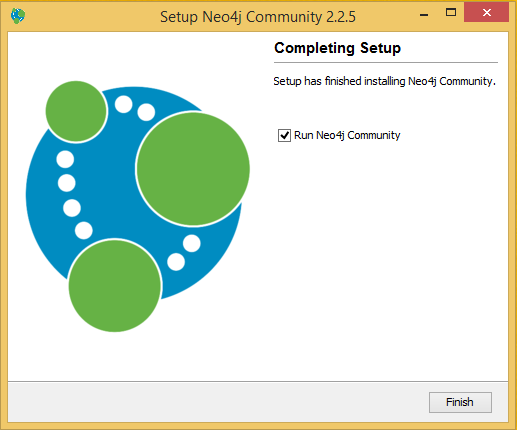
\includegraphics[scale=0.4]{./imagens/neo4j-install-step5.png}}
	\caption[Tela final de instalação do Neo4j]
	{Tela final de instalação do Neo4j. \textbf{Fonte:} Elaborado pelos autores.}
	\label{fig:exemplo1}
	
\end{figure}

\par A Figura 29 e 30 apresentam a tela inicial do banco de dados Neo4j e um exemplo de consulta realizada por meio da aplicação de gerencia da base de dados.

\begin{figure}[h!]
	\centerline{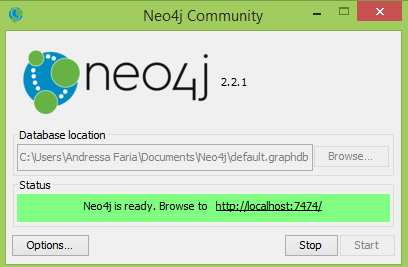
\includegraphics[scale=0.60]{./imagens/neo4j.jpg}}
	\caption[Tela de inicialização do Neo4j ]
	{Tela de inicialização do Neo4j \textbf{Fonte:} Elaborado pelos autores.}
	\label{fig:exemplo1}
\end{figure}

\begin{figure}[h!]
	\centerline{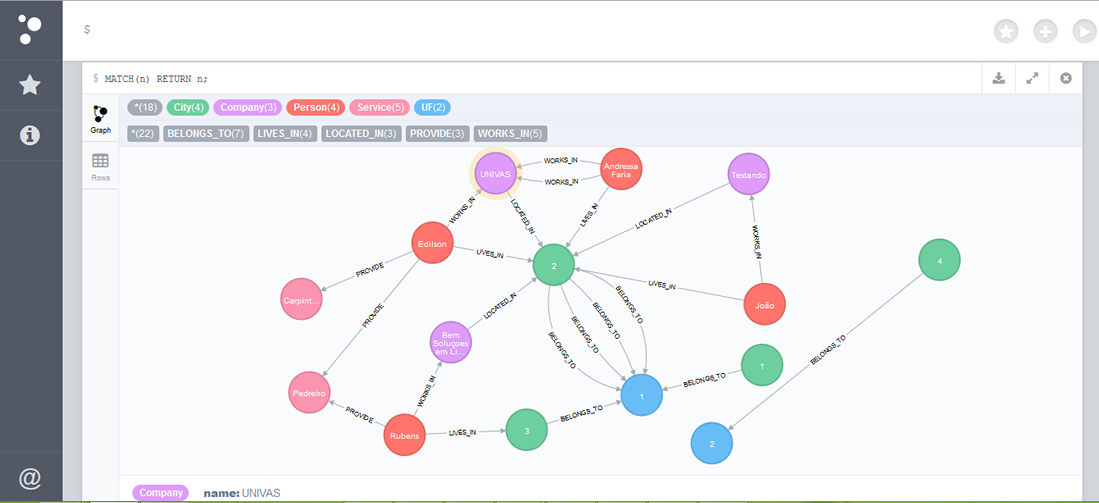
\includegraphics[scale=0.4]{./imagens/neo4j2.jpg}}
	\caption[Demonstração de uma consulta Cypher.]
	{Demonstração de uma consulta Cypher. \textbf{Fonte:} Elaborado pelos autores.}
	\label{fig:exemplo1}
\end{figure}
 
\newpage

\par Posterior a configuração do ambiente, iniciou-se o desenvolvimento propriamente dito. A princípio, utilizou-se as tecnologias Neo4j, sendo executado de forma \textit{embedded}, Primefaces e JSF. Porem não estava fluindo como o esperado, uma vez que o Neo4j utilizado desta maneira não permitia conectar ao sistema de gerenciamento da base de dados e abrir uma nova instancia de conexão simultânea, devido a limitações do próprio Neo4j, uma vez que um processo Java já ocupava tal conexão com o \textit{socket} do banco de dados.

\par Outro problema encontrado ao utilizar tais tecnologias foi que tanto a parte cliente (\textit{front end}) quanto a parte servidor (\textit{back end}) se encontravam totalmente acoplados em uma aplicação Java \textit{web}, portanto, a cada alteração realizada havia a necessidade de recompilar, construir e publicar a aplicação no servidor \textit{web}, impedindo que o desenvolvimento do \textit{software} fluísse, como era esperado. Por esses motivos decidiu-se mudar algumas das tecnologias utilizadas no \textit{front end} e, a maneira como o banco de dados era acessado até então. 

\par Posterior a esse incidente, passou-se a utilizar então as linguagens HTML 5, CSS 3, Java Script e Angular JS para auxiliar no desenvolvimento do \textit{front end}, ao invés de Primefaces e JSF. Para acesso ao banco de dados, lançou-se mão da forma \textit{embedded} e passou-se a utilizar a API REST disponibilizada pelo próprio banco. Tais decisões nos permitiram desacoplar o sistema e manter o \textit{front end} e o \textit{back end} independentes, evitando assim, que o mesmo problema voltasse a ocorrer.

\par Como a forma de conexão ao banco de dados foi alterada, houve-se a necessidade de reescrever a classe responsável por realizar esta conexão. Ao utilizar esta nova abordagem de conexão ao banco de dados, foi necessário informar o \textit{hostname} e a porta IP cujo banco está instalado e o diretório onde os dados estão localizados internamente no Neo4j. Neste trabalho foi utilizado o diretório padrão (/db/data). Após realizada esta configuração, foi necessário acrescentar o parâmetro ''/cypher'' à criação da instância de conexão, a fim de utilizar a API \textit{Cypher} em conjunto com esta nova abordagem, conforme apresenta a Figura 31.

\begin{figure}[h!]
	\centerline{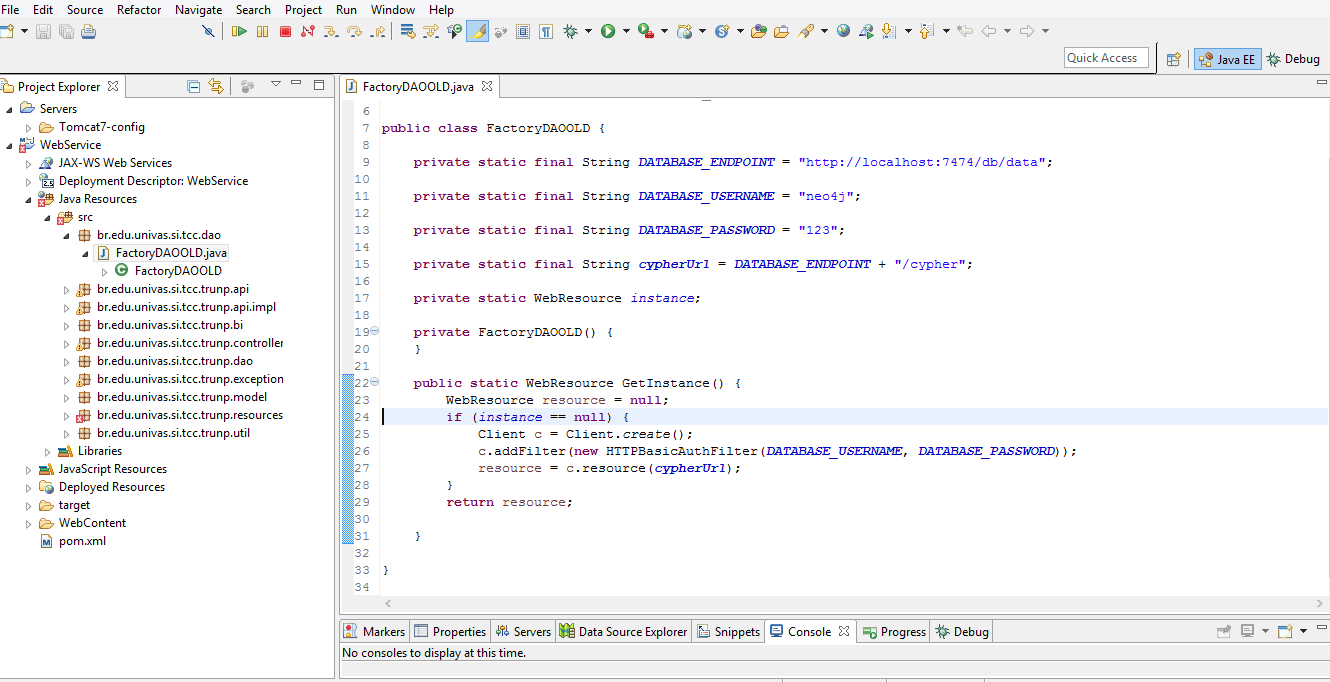
\includegraphics[scale=0.35]{./imagens/conexao-banco.jpg}}
	\caption[Código de comunicação com o banco]
	{Código de comunicação com o banco \textbf{Fonte:} Elaborado pelos autores.}
	\label{fig:exemplo1}
\end{figure}

\par Após realizar a mudança de tecnologias, foi necessário realizar alguns testes para compreender o funcionamento do \textit{web service} REST e paralelamente foi feito o levantamento de materiais de referência do \textit{framework} Angular JS. Foi preciso realizar testes para validar a conexão com o banco de dados Neo4j via API REST, fornecida por ele. Também foram realizados testes para envio de requisições e recebimento de respostas do \textit{web service} REST, utilizando o Angular JS. Para validar a conexão ao banco de dados via API REST foi necessário desenvolver algumas consultas em \textit{cypher} como apresenta a Figura 32.

\newpage
\begin{figure}[h!]
	\centerline{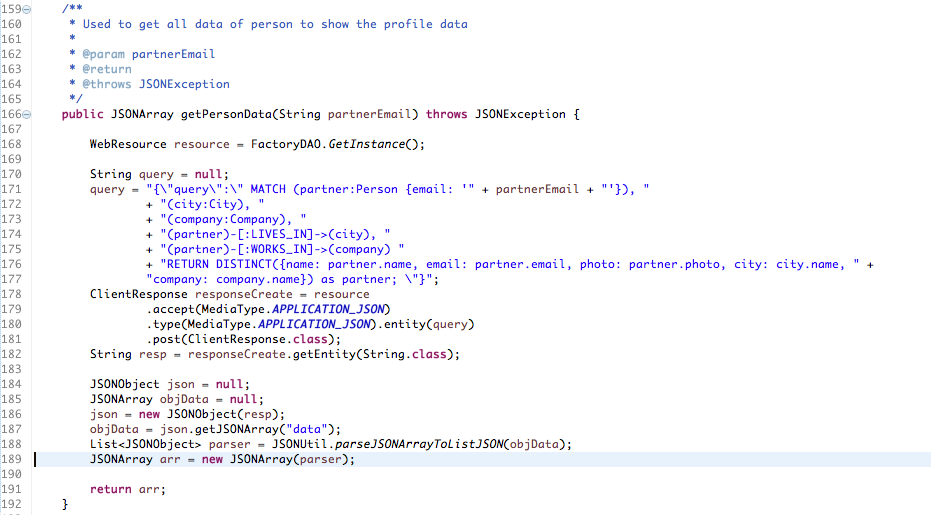
\includegraphics[scale=0.45]{./imagens/query-cypher.png}}
	\caption[Exemplo de consulta usando a API \textit{cypher}]
	{Exemplo de consulta usando a API \textit{cypher}. \textbf{Fonte:} Elaborado pelos autores.}
	\label{fig:exemplo1}
\end{figure}

\par Ao realizar estes testes foi constatado que seria necessário desenvolver uma maneira de converter os resultados das buscas realizadas no banco de dados Neo4j que, por padrão não retorna os resultados no formato JSON comum para um JSON válido, portanto, houve-se a preocupação em tratar estas respostas, a fim de retornar um JSON válido ao usuário que futuramente viria a utilizar a API REST fornecida por este \textit{software}. É possível visualizar este tratamento na Figura 32. 
 
\par A partir deste ponto, a aplicação estava totalmente desacoplada, sendo necessário realizar uma configuração, a fim de permitir que as requisições enviadas pelo \textit{front end} fossem aceitas pelo \textit{back end}, localizado em outro domínio.

\par Devido a mudança de tecnologias já comentadas, houve-se a necessidade de atualizar os diagramas de sequencia e de classe, inserindo os contratos de serviços do \textit{web service} REST. Com a definição deste contrato, deu-se início ao desenvolvimento dos casos de uso, identificados na primeira fase do ICONIX. 

\par Posterior a realização dos testes e da escolha definitiva da arquitetura que seria utilizada, iniciou-se a implementação dos casos de uso. O primeiro a ser implementado foi o caso de uso de criação de conta. Para este caso de uso, teve-se o cuidado de criar um mecanismo de criptografia de dados sigilosos, como usuário e senha, visando garantir a segurança da aplicação. Estas informações criptografadas são enviadas a cada requisição e validadas pelo \textit{web service}, sendo atualizadas caso sejam válidas, tornado mais complexo a quebra desta criptografia. Este mecanismo foi desenvolvido com base no sistema de \textit{login} via \textit{token}. Segundo o embasamento usado na criação de contas, deu-se início ao desenvolvimento do sistema de \textit{login} e \textit{logoff}, que também utilizam o conceito de criptografia via \textit{token}. 

Imagem tela de login

\par Com o funcionamento do sistema de login, passou-se a desenvolver a página inicial da aplicação. Esta página contém as informações que são restritas ao usuário cadastrado, podendo ser eles: contratantes, provedores de serviço ou ambos. O sistema apresenta uma página inicial diferente para cada tipo de conta, contendo apenas as informações que são liberadas de acordo com o acesso do usuário, sendo essas informações relatórios, últimas atualizações na rede de parceiros, avaliações de serviços e prováveis parceiros.

imagem das 3 contas.

\par O caso de uso localizar parceiros foi desenvolvido após a conclusão do caso de uso criar conta. A lógica deste caso de uso consiste em localizar os possíveis parceiros, com base na rede de parceria do contrante.

imagem localizar parceiro



\par Ainda relacionado ao tipo de conta contratante ou ambos, foi implementado o caso de uso adicionar parceiro, que permite ao usuário convidar um possível parceiro para fazer parte da sua rede. Após a implementação da lógica para adicionar um novo parceiro, houve-se a necessidade de implementar o serviço de requisições de parcerias, uma vez que não bastava apenas um contratante convidar outro para se tornarem parceiros, mas sim que o contratante convidado aceitasse sua solicitação de parceria, para assim se tornarem parceiros. Visando disponibilizar estas solicitações de forma agradável ao usuário, foi desenvolvida uma funcionalidade para que o usuário pudesse aceitar ou rejeitar a solicitação enviada à ele.

imagem aqui :D

\par Após realizada a implementação do caso de uso adicionar parceiro, houve-se a necessidade de desenvolver a busca por todos os usuário que possuiam o tipo de conta contratante ou ambos e que possuiam um relacionamento de parceria com o usuário autenticado no sistema, além da funcionalidade de localizar novos parceiros, baseando-se na localização da empresa na qual o usuário trabalha e na cidade onde ele vive, sempre ordenando os resultados por meio da quantidade de parceiros em comum. 

\par O caso de uso gerenciar serviços foi implementado em sequência, abrangendo as principais funcionalidaes de gerenciamento: cadastrar e adicionar um novo serviço ao usuário, cujo tipo de conta é provedor de serviços, listar os serviços atribuídos a ele, e remover serviços quando necessário. Visando melhorar a usabilidade, foi implementado um mecanismo de busca, que permitiu filtrar os resultados por meio de um campo que possui a função  auto completar, evitando assim, possíveis erros e diminuindo o tempo gasto pelo usuário para adicionar o serviço. A função realiza a busca em uma lista de serviços anteriormente cadastrados, no entanto, caso não haja o serviço solicitado, o usuário tem a liberdade de cadastrá-lo e atribuí-lo a si mesmo.

\par A partir deste ponto, foi possível iniciar o desenvolvimento do caso de uso localizar mão de obra, uma vez que, este caso de uso dependia diretamente das implementações das funcionalidades adicionar parceiros para os usuários contratantes e adicionar serviços aos provedores de serviço. Para facilitar a localização e deixar o \textit{software} mais usual, esta busca se basea inicialmente no serviço buscado pelo usuário, sendo posteriormente modificada para também levar em consideração a funcionalidade avaliar serviço que foi implementada paralelamente. A avaliação de serviço permite ao contratante dar uma nota ao serviço que foi prestado a ele. Com estas informações foi possível desenvolver uma busca que levaria em consideração, além destas informações, a rede de parceiros do usuário contratante, a fim de lhe apresentar as melhores opções possíveis.

\par A fim de abranger a busca e possibilitar que novos prestadores de serviços sejam avaliados pelos contratantes, a consulta que antes apresentava apenas provedores de serviços que possuiam avaliações, sendo elas, positivas ou negativas, foi ampliada, possibilitando que profissionais não avaliados também entrassem na lista de prováveis provedores de serviços.

\par Para auxiliar na tomada de decisão do usuário contratante, foi implementada uma funcionalidade que realiza o cálculo da média de um determinado serviço prestado por um usuário provedor de serviço, tomando como base as avaliações da rede de parceiros do usuário autenticado, da empresa onde ele trabalha e da cidade onde vive, oferecendo assim uma forma simples de ter acesso a qualidade do serviço prestado. *******************************

\par Após realizada todas as implementações já descritas, houve-se a preocupação de desenvolver uma interface, que além de amigável fosse prática ao usuário, desta forma, foi disponibilizada algumas informações relevantes, que auxiliam o usuário a compreender o que está ocorrendo em sua rede de parceria. Como exemplo é possível citar a lista de parceiros em comum entre o usuário autenticado no sistema e um determinado contratante por meio da página de perfil dele.

\par A fim de agregar mais funcionalidades para o usuário provedor de serviços, foi criado na página inicial do \textit{software} uma funcionalidade que visa apresentar algumas dicas interessantes que contribui com a sua imagem perante ao \textit{software}, levando-o assim a obter uma quantidade maior de oportunidades de trabalho.

\par Para finalizar o desenvolvimento foram desenvolvidos gráficos que apresentam ao usuário informações a respeito da qualidade do serviço prestado pelo provedor de serviços, comparando-os com os demais prestadores.

\par Realizado todos os procedimentos apresentados nesta sessão foi possível obter como resultado final a conclusão deste trabalho.

%\newpage
\section{Cronograma}

\par Será exibido aqui uma tabela contendo o cronograma a ser seguido por este projeto, desde a sua definição até a sua conclusão.

\begin{table}[htbp]
	\scriptsize
	\centering
	\begin{tabular}{|p{60mm}|p{3mm}|p{3mm}|p{3mm}|p{3mm}|p{3mm}|p{3mm}|p{3mm}|p{3mm}|p{3mm}|p{3mm}|p{3mm}|p{3mm}|}%Largura das colunas
		\hline\vspace{.99cm} %adicionando o espaçamento para que o nome dos meses caibam verticalmente
		\textbf{Ação} / \textbf{Mês} & 
		\parbox[t]{2mm}{\multirow{3}{*}{\rotatebox[origin=c]{90}{Janeiro}}} & \parbox[t]{2mm}{\multirow{3}{*}{\rotatebox[origin=c]{90}{Fevereiro}}} & 
		\parbox[t]{2mm}{\multirow{3}{*}{\rotatebox[origin=c]{90}{Março}}} & 
		\parbox[t]{2mm}{\multirow{3}{*}{\rotatebox[origin=c]{90}{Abril}}} &
		\parbox[t]{2mm}{\multirow{3}{*}{\rotatebox[origin=c]{90}{Maio}}} &
		\parbox[t]{2mm}{\multirow{3}{*}{\rotatebox[origin=c]{90}{Junho}}} &
		\parbox[t]{2mm}{\multirow{3}{*}{\rotatebox[origin=c]{90}{Julho}}} &
		\parbox[t]{2mm}{\multirow{3}{*}{\rotatebox[origin=c]{90}{Agosto}}} &
		\parbox[t]{2mm}{\multirow{3}{*}{\rotatebox[origin=c]{90}{Setembro}}} &
		\parbox[t]{2mm}{\multirow{3}{*}{\rotatebox[origin=c]{90}{Outubro}}} &
		\parbox[t]{2mm}{\multirow{3}{*}{\rotatebox[origin=c]{90}{Novembro}}} &
		\parbox[t]{2mm}{\multirow{3}{*}{\rotatebox[origin=c]{90}{Dezembro}}} \\
		\hline 
		Definição do Pré projeto & \cellcolor[HTML]{000000} &  &  &  &  &  &  &  &  &  &  & \\ \hline %1ª linha da tabela
		
		Aprovação do Pré projeto &  & \cellcolor[HTML]{000000} &  &  &  &  &  &  &  &  &  & \\ \hline %2ª linha
		
		Levantamento bibliográfico & \cellcolor[HTML]{000000} & \cellcolor[HTML]{000000} & \cellcolor[HTML]{000000} &  &  &  &  &  &  &  &  & \\ \hline %3ª linha
		
		Primeira entrega do Pré projeto &  & \cellcolor[HTML]{000000} &  &  &  &  &  &  &  &  &  & \\ \hline %4ª linha
		
		Orientação sobre Introdução &  & \cellcolor[HTML]{000000} &  &  &  &  &  &  &  &  &  & \\ \hline %5ª linha
		
		Entrega da Introdução &  & \cellcolor[HTML]{000000} &  &  &  &  &  &  &  &  &  & \\ \hline %6ª linha
		
		Orientações sobre Objetivos e Justificativas &  & \cellcolor[HTML]{000000} &  &  &  &  &  &  &  &  &  & \\ \hline %7ª linha
		
		Entrega dos Objetivos e Justificativas &  & \cellcolor[HTML]{000000} &  &  &  &  &  &  &  &  &  & \\ \hline %8ª linha
		
		Orientações sobre o Quadro Teórico &  & \cellcolor[HTML]{000000} & \cellcolor[HTML]{000000} &  &  &  &  &  &  &  &  & \\ \hline %9ª linha
		
		Entrega do Quadro Teórico &  &  & \cellcolor[HTML]{000000} &  &  &  &  &  &  &  &  & \\ \hline %10ª linha
		
		Orientações sobre o Quadro Metodológico &  &  & \cellcolor[HTML]{000000} & \cellcolor[HTML]{000000} &  &  &  &  &  &  &  & \\ \hline %11ª linha 
		
		Entrega do Quadro Metodológico &  &  &  & \cellcolor[HTML]{000000} &  &  &  &  &  &  &  & \\ \hline %12ª linha 
		
		Revisão de Referências &  &  &  & \cellcolor[HTML]{000000} & \cellcolor[HTML]{000000} &  &  &  &  &  &  & \\ \hline %13ª linha
		
		Qualificação do projeto  &  &  &  &  & \cellcolor[HTML]{000000} &  &  &  &  &  &  & \\ \hline %14ª linha
		
		Levantamento de requisitos &  &  &  &  & \cellcolor[HTML]{000000} & \cellcolor[HTML]{000000} &  &  &  &  &  & \\ \hline %15ª linha
		
		Desenvolvimento da pesquisa &  &  &  &  &  & \cellcolor[HTML]{000000} & \cellcolor[HTML]{000000}  & \cellcolor[HTML]{000000} & \cellcolor[HTML]{000000} & \cellcolor[HTML]{000000} & \cellcolor[HTML]{000000} & \\ \hline %16ª linha
	\end{tabular}
	\caption{Cronograma do desenvolvimento do projeto. \textbf{Fonte:} Elaborado pelos autores}
\end{table}

%\newpage
\section{Orçamento}

\par Abaixo serão apresentadas as despesas de forma geral previstas para a realização deste projeto.

\begin{table}[h]
	\begin{center}
	  	\rowcolors{1}{}{lightgray} %Deixar a tabela zebrada
  		\begin{tabular}{|l|c|}
  			\hline
  			%\cellcolor[HTML]{E6E4E4} 
  			\textbf{Despesas} & 
  			%\cellcolor[HTML]{E6E4E4} 
  			\textbf{Valor Previsto} \\
  			\hline
  			Impressão 				& R\$ 70,00 \\ \hline
  			Encadernação 			& R\$ 35,00 \\ \hline
  			Impressão em capa dura	& R\$ 80,00 \\ \hline
  			Livros 					& R\$ 1.700,00 \\ \hline
  			%\cellcolor[HTML]{E6E4E4} 120 + 200 + 200 + 80 + 160 + 210 + 150 + 95 + 160 + 180 + 145
  			\textbf{Total}			& 
  			%\cellcolor[HTML]{E6E4E4}
  			\textbf{R\$ 1.885,00} \\ \hline
  		\end{tabular}
  	\end{center}
  	\caption{Orçamento previsto do projeto. \textbf{Fonte:} Elaborado pelos autores}
\end{table}
